%%%%%%%%%%%%%%%%%%%%%%%%%%%%%%%%%%%%%%%%%
% Article EcoFoG
% Version 2.1 (23/10/2017)
%
% adapté de :
% Stylish Article
% LaTeX Template
% Version 1.0 (31/1/13)
%
% This template has been downloaded from:
% http://www.LaTeXTemplates.com
%
% Original author:
% Mathias Legrand (legrand.mathias@gmail.com)
%
% License:
% CC BY-NC-SA 3.0 (http://creativecommons.org/licenses/by-nc-sa/3.0/)
%
%%%%%%%%%%%%%%%%%%%%%%%%%%%%%%%%%%%%%%%%%


%----------------------------------------------------------------------------------------
%	PACKAGES AND OTHER DOCUMENT CONFIGURATIONS
%----------------------------------------------------------------------------------------

\documentclass[fleqn,10pt]{ArtEcoFoG} % Document font size and equations flushed left

\setcounter{tocdepth}{3} % Show only three levels in the table of contents section: sections, subsections and subsubsections


% Pandoc environments
\usepackage{framed}
\usepackage{fancyvrb}
\providecommand{\tightlist}{%
  \setlength{\itemsep}{0pt}\setlength{\parskip}{0pt}}
\newcommand{\VerbBar}{|}
\newcommand{\VERB}{\Verb[commandchars=\\\{\}]}
\DefineVerbatimEnvironment{Highlighting}{Verbatim}{commandchars=\\\{\}, fontsize=\scriptsize} % Code R
\definecolor{shadecolor}{RGB}{248,248,248}
\newenvironment{Shaded}{\begin{snugshade}}{\end{snugshade}}
\newcommand{\KeywordTok}[1]{\textcolor[rgb]{0.13,0.29,0.53}{\textbf{{#1}}}}
\newcommand{\DataTypeTok}[1]{\textcolor[rgb]{0.13,0.29,0.53}{{#1}}}
\newcommand{\DecValTok}[1]{\textcolor[rgb]{0.00,0.00,0.81}{{#1}}}
\newcommand{\BaseNTok}[1]{\textcolor[rgb]{0.00,0.00,0.81}{{#1}}}
\newcommand{\FloatTok}[1]{\textcolor[rgb]{0.00,0.00,0.81}{{#1}}}
\newcommand{\ConstantTok}[1]{\textcolor[rgb]{0.00,0.00,0.00}{{#1}}}
\newcommand{\CharTok}[1]{\textcolor[rgb]{0.31,0.60,0.02}{{#1}}}
\newcommand{\SpecialCharTok}[1]{\textcolor[rgb]{0.00,0.00,0.00}{{#1}}}
\newcommand{\StringTok}[1]{\textcolor[rgb]{0.31,0.60,0.02}{{#1}}}
\newcommand{\VerbatimStringTok}[1]{\textcolor[rgb]{0.31,0.60,0.02}{{#1}}}
\newcommand{\SpecialStringTok}[1]{\textcolor[rgb]{0.31,0.60,0.02}{{#1}}}
\newcommand{\ImportTok}[1]{{#1}}
\newcommand{\CommentTok}[1]{\textcolor[rgb]{0.56,0.35,0.01}{\textit{{#1}}}}
\newcommand{\DocumentationTok}[1]{\textcolor[rgb]{0.56,0.35,0.01}{\textbf{\textit{{#1}}}}}
\newcommand{\AnnotationTok}[1]{\textcolor[rgb]{0.56,0.35,0.01}{\textbf{\textit{{#1}}}}}
\newcommand{\CommentVarTok}[1]{\textcolor[rgb]{0.56,0.35,0.01}{\textbf{\textit{{#1}}}}}
\newcommand{\OtherTok}[1]{\textcolor[rgb]{0.56,0.35,0.01}{{#1}}}
\newcommand{\FunctionTok}[1]{\textcolor[rgb]{0.00,0.00,0.00}{{#1}}}
\newcommand{\VariableTok}[1]{\textcolor[rgb]{0.00,0.00,0.00}{{#1}}}
\newcommand{\ControlFlowTok}[1]{\textcolor[rgb]{0.13,0.29,0.53}{\textbf{{#1}}}}
\newcommand{\OperatorTok}[1]{\textcolor[rgb]{0.81,0.36,0.00}{\textbf{{#1}}}}
\newcommand{\BuiltInTok}[1]{{#1}}
\newcommand{\ExtensionTok}[1]{{#1}}
\newcommand{\PreprocessorTok}[1]{\textcolor[rgb]{0.56,0.35,0.01}{\textit{{#1}}}}
\newcommand{\AttributeTok}[1]{\textcolor[rgb]{0.77,0.63,0.00}{{#1}}}
\newcommand{\RegionMarkerTok}[1]{{#1}}
\newcommand{\InformationTok}[1]{\textcolor[rgb]{0.56,0.35,0.01}{\textbf{\textit{{#1}}}}}
\newcommand{\WarningTok}[1]{\textcolor[rgb]{0.56,0.35,0.01}{\textbf{\textit{{#1}}}}}
\newcommand{\AlertTok}[1]{\textcolor[rgb]{0.94,0.16,0.16}{{#1}}}
\newcommand{\ErrorTok}[1]{\textcolor[rgb]{0.64,0.00,0.00}{\textbf{{#1}}}}
\newcommand{\NormalTok}[1]{{#1}}
\usepackage{longtable,booktabs}
\usepackage{caption}
% These lines are needed to make table captions work with longtable:
\makeatletter
\def\fnum@table{\tablename~\thetable}
\makeatother
% longtable 2 columns
% https://tex.stackexchange.com/questions/161431/how-to-solve-longtable-is-not-in-1-column-mode-error
\makeatletter
\let\oldlt\longtable
\let\endoldlt\endlongtable
\def\longtable{\@ifnextchar[\longtable@i \longtable@ii}
\def\longtable@i[#1]{\begin{figure}[t]
\onecolumn
\begin{minipage}{0.5\textwidth}\scriptsize
\oldlt[#1]
}
\def\longtable@ii{\begin{figure}[t]
\onecolumn
\begin{minipage}{0.5\textwidth}\scriptsize
\oldlt
}
\def\endlongtable{\endoldlt
\end{minipage}
\twocolumn
\end{figure}}
\makeatother

\usepackage{graphicx,grffile}
\makeatletter
\def\maxwidth{\ifdim\Gin@nat@width>\linewidth\linewidth\else\Gin@nat@width\fi}
\def\maxheight{\ifdim\Gin@nat@height>\textheight0.8\textheight\else\Gin@nat@height\fi}
\makeatother
% Scale images if necessary, so that they will not overflow the page
% margins by default, and it is still possible to overwrite the defaults
% using explicit options in \includegraphics[width, height, ...]{}
\setkeys{Gin}{width=\maxwidth,height=\maxheight,keepaspectratio}

% User-adder preamble
\usepackage{textcomp} \DeclareUnicodeCharacter{B0}{\textdegree}
\usepackage{tabu} \usepackage{caption}
\captionsetup{justification = justified}
\renewenvironment{table}{\begin{table*}}{\end{table*}\ignorespacesafterend}
\hyphenation{bio-di-ver-si-ty sap-lings}

%----------------------------------------------------------------------------------------
%	ARTICLE INFORMATION
%----------------------------------------------------------------------------------------

\JournalInfo{Hal xxx} % Journal information
\Archive{DOI xxxx} % Additional notes (e.g. copyright, DOI, review/research article)

\PaperTitle{Post-Disturbance Tree Community Trajectories in a Neotropical Forest} % Article title

\Authors{
Ariane MIRABEL\textsuperscript{1*}\\ Eric Marcon\textsuperscript{1}\\ Bruno Hérault\textsuperscript{2 3}
} % Authors
\affiliation{
\textsuperscript{1}UMR EcoFoG, AgroParistech, CNRS, Cirad, INRA, Université des Antilles,
Université de Guyane.\\ \hspace{1em} Campus Agronomique, 97310 Kourou, France.\\\textsuperscript{2}Cirad, Univ montpellier, UR Forests \& Societies.\\ \hspace{1em} Montpellier, France.\\\textsuperscript{3}INPHB, Institut National Polytechnique Félix Houphouet-Boigny\\ \hspace{1em} Yamoussoukro, Ivory Coast.
}
\affiliation{*\textbf{Corresponding author}: ariane.mirabel@ecofog.gf, http://www.ecofog.gf/spip.php?article47} % Corresponding author

\Keywords{mot-clés, séparés par des virgules} % Keywords - if you don't want any simply remove all the text between the curly brackets
\newcommand{\keywordname}{Keywords} % Defines the keywords heading name

%----------------------------------------------------------------------------------------
%	ABSTRACT
%----------------------------------------------------------------------------------------

\Abstract{
Résumé de l'article.
}

%----------------------------------------------------------------------------------------

\usepackage{amsthm}
\newtheorem{theorem}{Theorem}[section]
\newtheorem{lemma}{Lemma}[section]
\theoremstyle{definition}
\newtheorem{definition}{Definition}[section]
\newtheorem{corollary}{Corollary}[section]
\newtheorem{proposition}{Proposition}[section]
\theoremstyle{definition}
\newtheorem{example}{Example}[section]
\theoremstyle{definition}
\newtheorem{exercise}{Exercise}[section]
\theoremstyle{remark}
\newtheorem*{remark}{Remark}
\newtheorem*{solution}{Solution}
\begin{document}

\selectlanguage{english}

\flushbottom % Makes all text pages the same height

\maketitle % Print the title and abstract box

\tableofcontents % Print the contents section

\thispagestyle{empty} % Removes page numbering from the first page

%----------------------------------------------------------------------------------------
%	ARTICLE CONTENTS
%----------------------------------------------------------------------------------------
























\section{Introduction}\label{introduction}

The large areas covered with tropical forests worldwide hold crucial
economic, social and cultural value. They provide wood and multiple
non-timber forest products, shelter a diversified fauna, regulate the
local climate, support the carbon, water and nutrient cycles, and ensure
cultural and human well-being. The simultaneous increase of forests
products demand and substantial climatic changes currently heighten the
pressure on the remaining forests
\citep{Gibson2011a, Morales-Hidalgo2015}. It threatens the maintenance
of communities structure, composition and functioning and the underlying
dynamics in space and time \citep{Anderson-Teixeira2013, Sist2015}.

In tropical forest, ecological communities are contantly re-shaped by
the natural disturbance events that changes the abiotic environment,
through the fluxes of light, heat and water, and the biotic interaction
and competitive pressure \citep{Goulamoussene2017}. The cornerstone of
tropical forests ecology is then to understand the underlyings of
ecosystem response to disturbance, its mechanisms and drivers
\citep{White2001, Chazdon2003a}. For now, this has been largely studied
through structural parameters, rapid and convenient to measure, as
aboveground biomass, tree height or stem density
\citep{Piponiot2016, Rutishauser2016}. These structural parameters have
then been sucessfully modeled and allowed to assess the maintenance of
ecosystems processes and services \citep{Denslow2000, Blanc2009}.
However the response of tree species diversity remains unclear, also it
is determinant of ecosystems productivity, stability and functioning
\citep[\citet{Liang2016}]{Tilman2014} and would be most probably
impacted by post-disturbance environmental changes
\citep{Baraloto2012a}.

In the short-term disturbance demonstrated negligible or even positive
impacts on communities diversity, which have been formalized by the
intermediate disturbance hypothesis (IDH) stating a maximized species
diversity at intermediate disturbance intensity
\citep{Molino2001, Kariuki2006a, Berry2008a}. Validations of the IDH in
the long term, however, remain scarce and mainly rely on the analysis of
the rough species richness that gives limited or misleading information
on forests recovery and functioning \citep{Martin2015, Chaudhary2016}.
More releveant monitoring would encompass communities composition, that
is crucial for conservation issues, and diversity profiles, that reveals
ecological rules underlying communities' structure
\citep{Magurran1988, Lavorel2002, Bellwood2006}. Furthermore, the
functional approach accounting for differenes species biological
attributes would be insightful as it reveals the species role in the
post-disturbance trajectory of ecosystems functioning
\citep{Violle2007b, Moretti2009, Baraloto2012a, Scheiter2013}. In that
respect major functional traits related to species ecology and
performance were largely adopted through an integrative framework
\citep{Diaz2005, Villeger2008a}. The functional trait-based approach,
for example, highlighted in tropical rainforests the environmental
filters fostering disturbance resistant species with rapid growth and
efficient resources acquisition \citep{Molino2001, Haddad2008}. In
disturbed tropical rainforests, this framework translates into the
fostering of disturbance resistant species with rapid growth and
efficient resources acquisition \citep{Molino2001, Haddad2008}. It
results in a shift from ``conservative'' slow-growing species dealing
with scarce resources that dominate before disturbance, to
``acquisitive'' fast-growing species with rapid and efficient use of
abundant resources \citep{TerSteege2001, Reich2014, Herault2011}. It was
mirrored by shifts in key functional traits related to resource
acquisition (leaf area, density and chlorophyll content, and stem
specific gravity and bark thickness), tree growth and reproduction life
history traits (seed mass and maximum height)
\citep{Wright2004, Westoby2006a, Chave2009b}.

A proper monitoring of communities response should therefore encompass
taxonomic and functional diversity and composition measures to test the
validity of the IDH in the long term for tropical forests, and clarify
the resilience of communities evenness, composition, and also
functioning. The trajectories followed by all these facets would
highlight the role of deterministic processes, like competitive
exclusion or abiotic selection, and the communities' convergence
maintaining intrinsinc differences in diversity and composition,which is
as much insgights for future adaptive conservation strategies
\citep{Adler2007}.

Here we investigated over 30 years the response of 75 ha of forests
plots set up on a gradient of disturbance intensity, from 10 to 60\% of
ecosystem biomass removed. We made use of a large functional traits
database browsing major leaf, stem and seed traits and species maximum
height to draw the trajectories over time of communities taxonomic and
functional composition and diversity. Specifically, we (i) tested the
validity of the IDH in the long term for tropical hyperdiverse forest
and highlighted the ecological rules shaping their response to
disturbance, (ii) clarified the different facets of communities
resilience in terms of communities composition, diversity and
functioning \emph{????(iii) questioned the completeness of communities
recovery given the altered functional redundancy.}

\section{Material and Methods}\label{material-and-methods}

\subsection{Study site}\label{study-site}

Paracou station in French Guiana (5°18'N and 52°53'W) is located in a
lowland tropical rain forest corresponding to a tropical wet climate
with mean annual precipitation averaging 2980 mm.y\textsuperscript{-1}
(30-y period) with a 3-month dry season (\textless{} 100
mm.month\textsuperscript{-1}) from mid-August to mid-November, and a
one-month dry season in March \citep{Wagner2011}. Elevation ranges
between 5 and 50 m and mean annual temperature is 26°C. Soils correspond
to thin acrisols over a layer of transformed saprolite with low
permeability generating lateral drainage during heavy rains. The
experiment corresponds to a network of twelve 6.25ha plots that have
undergone a gradient of three logging, thinning and fuelwood treatments
(Table \ref{tab:Tab1}). Disturbance treatments were attributed according
to a randomized plot design with three replicate blocks of four plots.
The disturbance corresponds to averages of 10 trees removed per hectare
with a diameter at 1.3 m height (DBH) above 50 cm for treatment 1 (T1),
32 trees/ha above 40 cm DBH for treatment 2 (T2) and 40 trees above 40
cm DBH for treatment 3 (T3). Treatments T2 and T3 besides included the
thinning of trees by poison girdling \citep{Blanc2009}. The disturbance
intensity was measured as the percentage of aboveground biomass (\%AGB)
lost between the first inventory in 1984 and five years after
disturbance (ref to be found). Biomass measurements were performed with
the BIOMASS package R package \citep{Biomass2018}.

\begin{table}

\caption{\label{tab:Tab1}Intervention table, summary of the disturbance intensity for the 4 plot treatments in Paracou.}
\centering
\begin{tabu} to \linewidth {>{\raggedright}X>{\raggedright}X>{\raggedright}X>{\raggedright}X>{\raggedright}X}
\toprule
Treatment & Timber & Thinning & Fuelwood & \%AGB lost\\
\midrule
Control &  &  &  & 0\\
T1 & DBH $\geq$ 50 cm, commercial species, $\approx$ 10 trees/ha &  &  & $[12\%-33\%]$\\
T2 & DBH $\geq$ 50 cm, commercial species, $\approx$ 10 trees/ha & DBH $\geq$ 40 cm, non-valuable species, $\approx$ 30 trees/ha &  & $[33\%-56\%]$\\
T3 & DBH $\geq$ 50 cm, commercial species, $\approx$ 10 trees/ha & DBH $\geq$ 50 cm, non-valuable species, $\approx$ 15 trees/ha & 40 cm $\leq$ DBH $\leq$ 50 cm, non-valuable species, $\approx$ 15 trees/ha & $[35\%-66\%]$\\
\bottomrule
\end{tabu}
\end{table}

\subsection{Inventories protocol and dataset
collection}\label{inventories-protocol-and-dataset-collection}

The study site corresponds to a tropical rainforest with a dominance of
Fabaceae, Chrysobalanaceae, Lecythidaceae and Sapotaceae botanical
families. In the twelve experimental plots of the experiment, all trees
above 10 cm DBH were mapped and measured annually since 1984. During
inventories, trees were first identified with a vernacular name assigned
by the field team, and afterward with a scientific name assigned by a
botanist during regular botanical campaigns. In 1984, specific
vernacular names were given to 62 commercial or common species whereas
other less common species were identified under two identifiers only
separating trees and palm trees. The botanical campaigns carried every 5
to 6 years to identify all trees at the species level only started in
2003 and identification practices varied among plots and successive
campaigns. This raised methodological issues as vernacular names usually
correspond to different botanical species, resulting in significant
taxonomic uncertainties that had to be propagated to composition and
diversity metrics through a Bayesian framework. The uncertainty
propagation was done by the replenishment of inventories completed at
genus level from real incomplete ones on the basis of
vernacular/botanical names association.

Vernacular names were replaced through multinomial trials
\(M_v\Big(\big[s_1, s_2, …, s_N\big],\big[\alpha_1, \alpha_2,…, \alpha_3\big]\Big)\)
based on the observed association probability
\(\big[\alpha_1, \alpha_2,…, \alpha_3\big]\) between each vernacular
name \emph{v} and the species \(\big[s_1, s_2, …, s_N\big]\) recorded in
the inventory. See appendix 1 and \citet{Aubry-Kientz2013} for the
detailed methodology.

The functional diversity metrics used a dataset for 6 functional traits
representing leaf economics (leaves thickness, toughness, total
chlorophyll content and specific leaf area, the leaf area per unit dry
mass) and wood economics (wood specific gravity and bark thickness), and
life history traits (maximum specific height and seed mass).

The trait database came from the BRIDGE project \footnote{http://www.ecofog.gf/Bridge/}
where trait values were assessed from a selection of individuals located
in nine permanent plots in French Guiana, including two in Paracou.
Missing trait values were filled using multivariate imputation by
chained equation (mice) restricted to samples pertaining to the next
higher taxonomic level, in order to account for the phylogenetic signal
of the functional traits. The dataset comprised 294 botanical species
pertaining to 157 botanical genera.

Whenever a species inventoried was not in the dataset, it was attributed
a set of traits values randomly sampled among species of the same next
higher taxonomic level. As seed mass information corresponds to a
classification into mass classes, no data filling process was applied so
analysis were performed considering the 414 botanical species of the
seed mass dataset. All composition and diversity metrics corresponded to
the average obtained after 50 iterations of the taxonomic uncertainty
propagation framework and of the filling process of missing trait
values.

\subsection{Composition and diversity
metrics}\label{composition-and-diversity-metrics}

To counter the remaining taxonomic uncertainty, plots taxonomic
composition and diversity were analysed at the genus level, \emph{i.e.}
referring to the genus of observed or trialed botanical names.
Variations in plots taxonomic and functional composition after
disturbance was visualized by their trajectories over 30 years in a
two-dimensional ordination space. Two NMDS were conducted, either from
taxonomic flora inventories or from plots functional composition based
on the 7 leaf, stem and life history traits (without seed mass classes).
In both cases the NMDS were performed using occurrence-based (Jaccard)
as well as abundance-based (Bray-Curtis) dissimilarity measures.
Trajectories along time were reported through the euclidean distance of
successive inventories to the reference inventories in 1989, 5 years
after disturbance, when the uncertainty degree did not exceed 30\% of
undetermined trees. The trajectories of the leaf and stem and life
traits were also visualized with the community weighted means (CWM),
representing the average trait value in a community weighted by relative
abundance of the species carrying each value
\citep{Diaz2007, Garnier2004}. To compensate the intrinsinc difference
among plots the trajectories corresponded to the differences along time
with the reference inventory in 1989. Species seed mass corresponded to
5 classes of increasing mass, seed mass trajectories were therefore
reported as the proportion of each class in the inventories.

The taxonomic diversity was assessed through Richness and the Hill
number translation of Shannon and Simpson indices \citep{Hill1973}.
These three indices belong to the set of HCDT or generalized entropy,
respectively corresponding to the 0, 1 and 2 order of diversity (q),
which proved well suited for diversity studies
\citep{Patil1982, Tothmeresz1995}. The functional diversity was reported
using the Rao index of quadratic entropy which combines species
abundance distribution and average pairwise dissimilarity based on all
functional and life traits.

The functional redundancy was measured as the overlap among species in
communities' functional space \citep{Carmona2016}. The samples of the
trait database were first located with a PCA analysis in a
two-dimensional functional space summarizing the 8 functional traits
considered. We choose to summarize species functional space through a
PCA because functional traits considered were already somehow redundant
and allows not to overweight the role of one trait. Then, multivariate
kernel density estimator associated with individual trees were summed to
give the distribution of traits probabilites of each species. For each
community the trait probability distributions of corresponding species
were combined and weighted by species abundance. Eventually communities
functional redundancy was measured as the sum of overlap between species
weighted functional density. Communities functional redundancy is
expressed as the average number of species that could be removed from
the community without reducing the functional space.

\section{Results}\label{results}

\subsection{Communities Diversity}\label{communities-diversity}

Communities taxonomic diversity trajectories were examined through the
Richness, Shannon and Simpson diversities at genus level, in relation to
the 1989 inventories (5 years after disturbance) (See annexe I). For
undisturbed plots the Richness, Shannon and Simpson diversities remained
stable over the 30 years monitored. After low disturbance intensity the
richness increased, reaching a maximum gain of 14 botanical genera (plot
3 from treatment 2). After intense disturbance, plots taxonomic richness
followed unimodal trajectories first decrease for around ten years and
then increasing to return to pre-disturbance values. For all disturbed
plots the taxonomic evenness (Shannon and Simpson diversities)
increased, following unimodal trajectories with a just beginning return
towards initial values after 30 years. The maximum evenness, reached
after around 20 years, was positively correlated to the disturbance
intensity (\(\rho_{spearman}^{Shannon}=0.86\), and
\(\rho_{spearman}^{Simpson}=0.89\)). Only two T3 plots (plots 8 and 12)
were still increasing 30 years after disturbance \ref{fig:IDHplot},
suggesting similar but delayed trajectories.

Communities functional diversity trajectories were examined through the
Rao diversity based on the 7 leaf, stem and life history traits (the
seed mass was excluded as a qualitative variable). The plot 7 from
treatment 1 displayed a constantly outlying diversity and was removed
from the graphical representation for better readability (see appendix
for full graphs). The functional diversity of all undisturbed
communities remained stable along the 30 years. For all disturbed
communities the functional diversity followed unimodal trajectories with
a return towards the initial state, comparable to the control plots.

The impact of disturbance was examined specifically through the linear
correlation between the disturbance intensity (intial \%AGB removed) and
the Simpson and Rao diversities (diversities of order 2) at three focus
times after disturbance (10, 20 and 30 years) \ref{fig:IDHplot}. The
Simpson diversity was weakly related to the disturbance intensity
(\(R^2<0.25\)) and only from 20 years after disturbance. The Rao
diversity was more strongly correlated to the disturbance intensity
(\(0.55<R^2<0.75\)) for the three times studied. The impact of
disturbance, translated by the slope of the linear correlation, was the
highest 20 years after disturbance.

\begin{figure*}

{\centering 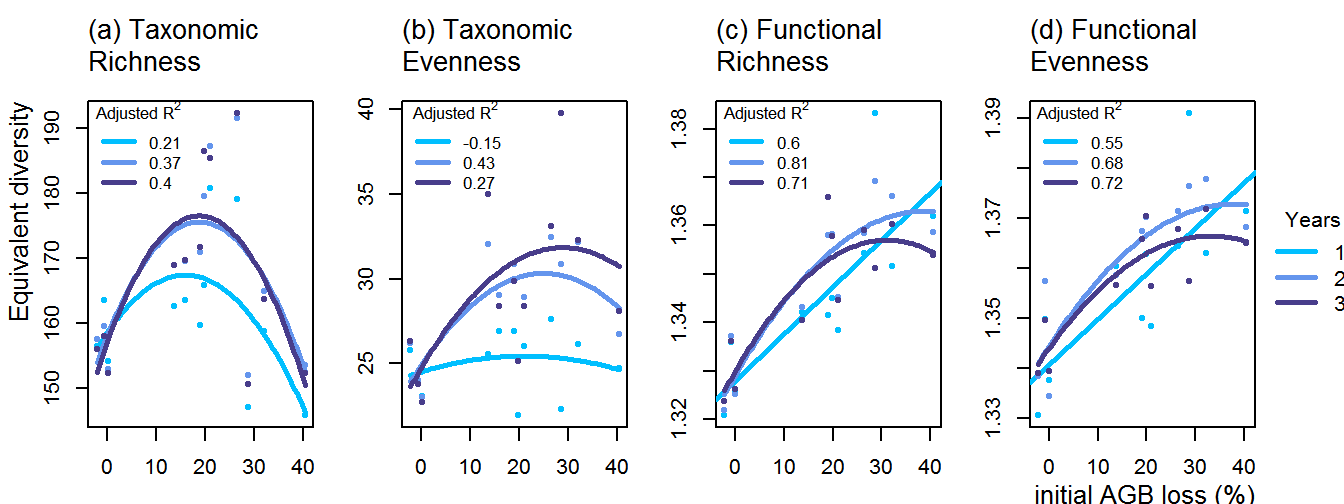
\includegraphics[width=1\linewidth]{WholePlotTrajectories_files/figure-latex/IDHplot-1} 

}

\caption{Upper panels, Trajectories of the Simpson taxonomic diversity \textbf{(a)} and Rao functional diversity \textbf{(b)} over 30 years after disturbance, corresponding to the median and 0.025 and 0.975 percentile observed after 50 iteration of the taxonomic uncertainty propagation and the missing trait value filling processes. Initial treatments are represented by solid lines colors with green for control, blue for T1,orange for T2 and red for T3. Lower panels, Relationship between the initial \%AGB removed and the median values of Simpson \textbf{(c)} and Rao \textbf{(d)} diversities at three times after disturbance. Solid lines colors represent the time, 10 years (yellow), 20 years (orange) and 30 years (brown) after disturbance.}\label{fig:IDHplot}
\end{figure*}

\subsection{Communities composition}\label{communities-composition}

\subsubsection{Taxonomic and functional
trajectories}\label{taxonomic-and-functional-trajectories}

In the inventories from 1989 (5 years after disturbance) to 2015 (31
years after disturbance), 828388 trees and 591 botanical species
pertaining to 223 genus and 64 botanical families were recorded. The
trajectories of taxonomic and functional composition were visualized in
a two dimensional ordination space mapping the successive inventories
according to their flora and the corresponding traits. Classifications
were performed using either abundance-based Bray-Curtis (Figure
\ref{fig:NMDSplans}) or incidence-based Jaccard dissimilarity. Both
metrics gave similar results, so only analysis using Bray-Curtis
dissimilarity will be discussed here.

While both taxonomic and functional composition remained stable in
undistrubed communities, after disturbed they followed consistent
trajectories over time that revealed significant compositional changes.
Considering the mapping of functional traits in the same dimensional
space, the post-disturbance trajectories corresponded to shifts towards
more acquisitive functional strategies: disturbed communities changed
from high average WD to high average SLA and chlorophyll content. For
disturbed communities the distance of successive inventories to the
reference inventory in 1989 followed unimodal trajectories (AppendixI,
Figure A2). The maximum of communities dissimilarity to their initial
state was positively correlated to the disturbance intensity for both
taxonomic and functional composition
(\(\rho_{spearman}^{taxonomic}=0.91\) and
\(\rho_{spearman}^{functional}=0.96\) respectively). The time at maximum
dissimilarity was reached around 26 years after disturbance for
taxonomic composition and 22 years for functional composition. All
trajectories followed cyclic composition changes with a return towards
the initial composition (Figure \ref{fig:NMDSplans}).

\begin{figure*}

{\centering 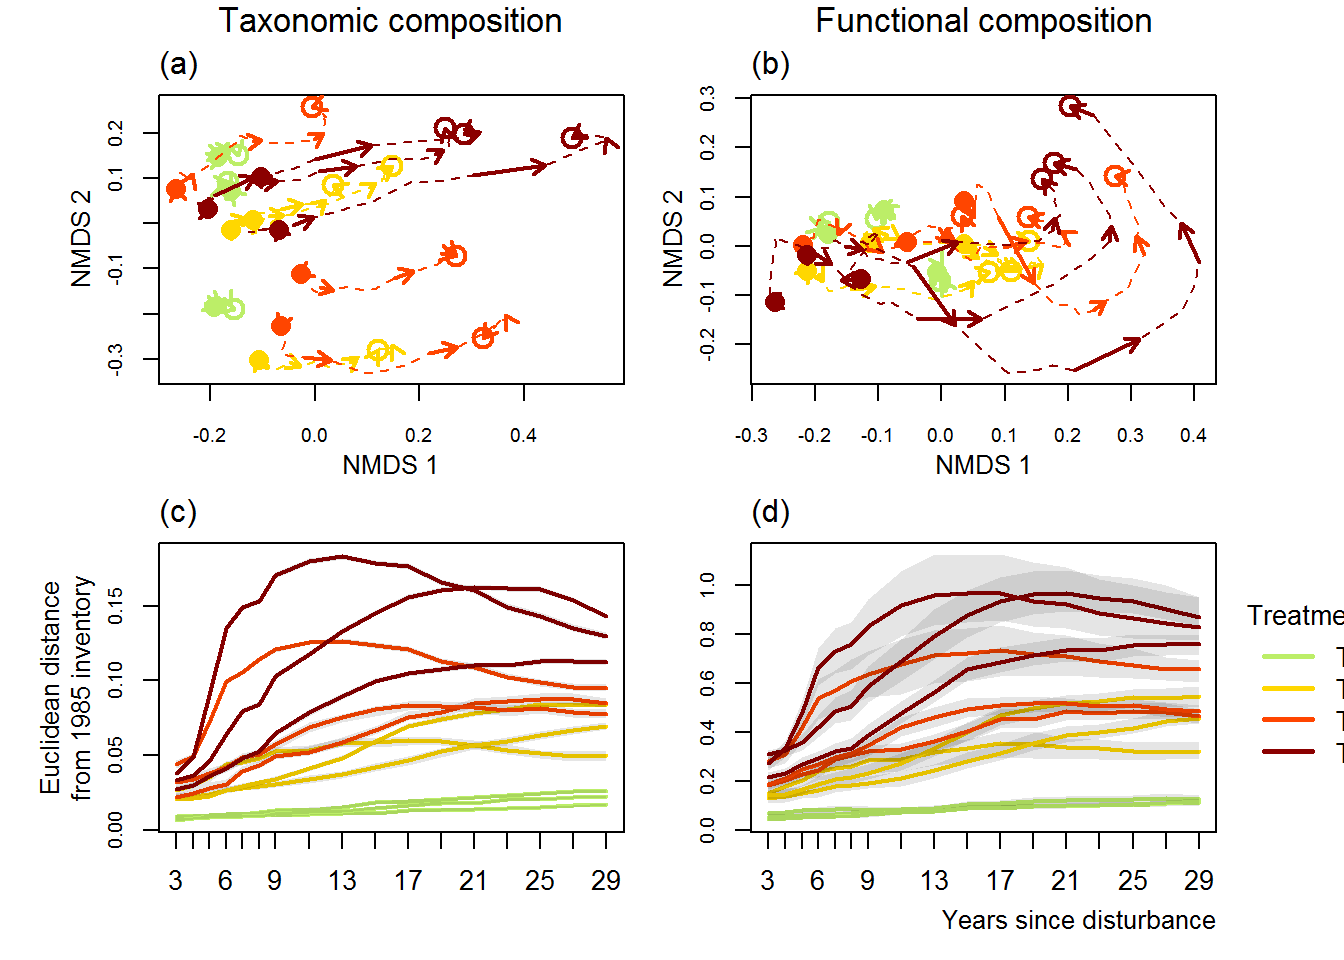
\includegraphics[width=1\linewidth]{WholePlotTrajectories_files/figure-latex/NMDSplans-1} 

}

\caption{Trajectories of the plots in terms of flora composition (left panels \textbf{(a)} and \textbf{(c)}) and functional composition (right panels \textbf{(b)} and \textbf{(d)}) regarding the 6 leaf and stem functional traits, the maximum allometric height and seed mass class. Plots trajectories are first represented in the two-dimensional space from the NMDS performed for the 30 years after disturbance based on Bray-Curtis dissimilarity measures between successive inventories (Upper panels \textbf{(a)} and \textbf{(b)}). Then the lower panels (\textbf{(c)} and \textbf{(d)}) represent the euclidean distance to initial condition along the 30 sampled years. Line colors represent the disturbance treatment (green for control, blue for T1,orange for T2 and red for T3). The 0.025 and 0.975 percentile correspond to the variance observed for 50 iteration of the taxonomic uncertainty propagation and functional trait filling processes.}\label{fig:NMDSplans}
\end{figure*}

\subsubsection{Traits community weighted means
(CWM)}\label{traits-community-weighted-means-cwm}

The changes observed in plots functional composition went hand to hand
with consistent trajectories of the 8 functional and life history traits
visualized through plots community weighted means (CWM) (Figure
\ref{fig:CWM}) of the leaves thickness, chlorophyll content, toughness
and specific area, wood specific gravity, bark thickness, seed mass and
maximum adult height.

Except for leaf chlorophyll content, which continued to increase for
some T3 and T2 plots, all traits and seed mass proportions followed a
unimodal trajectories and either stabilized or returned towards their
initial values 30 years after disturbance. At that time the weighted
means of communities specific maximum height at adult stage
(\emph{Hmax}), leaf toughness (\emph{L\_toughness}) and wood specific
gravity (\emph{WD}) remained significantly lower than their initial
value and than these of the control plots (Figure \ref{fig:CWM}). The
weighted means of bark thickness (\emph{Bark\_thick}) similarly remained
substantilly higher than initially for all disturbed plots while the
specfic leaf area (\emph{SLA}) had almost recovered its initial value,
similar as those of undisturbed plots. For all traits the maximum
difference to initial state was correlated to the disturbance intensity
(\(\rho_{spearman}^{L_{thickness}}=0.67\),
\(\rho_{spearman}^{L_{chloro}}=0.45\),
\(\rho_{spearman}^{L_{toughness}}=-0.43\),
\(\rho_{spearman}^{SLA}=0.93\), \(\rho_{spearman}^{WD}=-0.78\),
\(\rho_{spearman}^{Bark-thickness}=0.88\),
\(\rho_{spearman}^{Hmax}=-0.48\)).

\begin{figure*}

{\centering 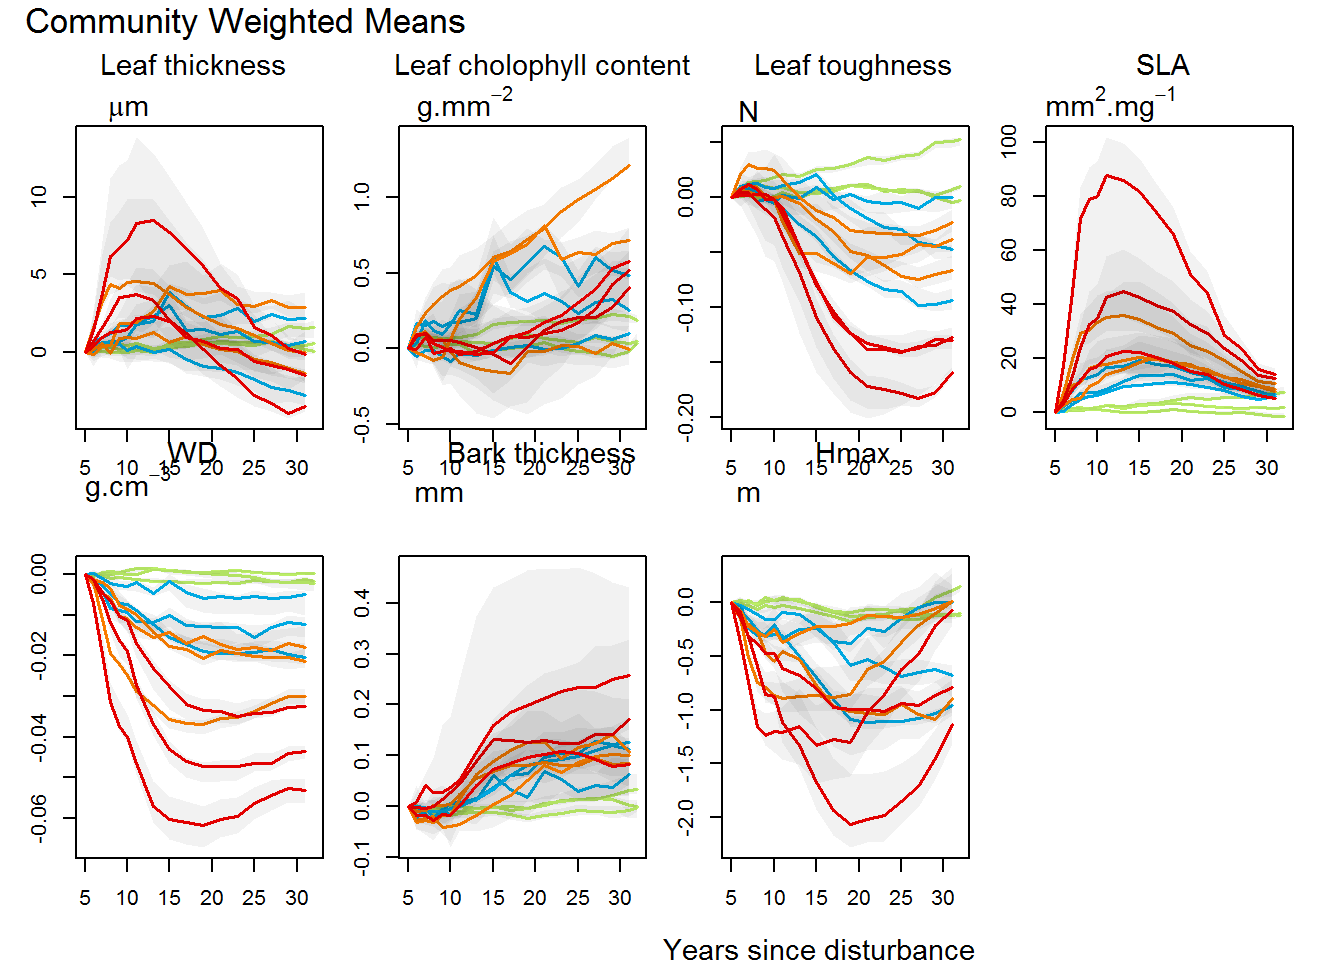
\includegraphics[width=1\linewidth]{WholePlotTrajectories_files/figure-latex/CWM-1} 

}

\caption{Trajectories of the communities weighted means (CWM) over 30 years after disturbance of 4 leaf traits (Leaf thickness, \emph{L\_thickness}, chlorophyll content, \emph{L\_chloro}, toughness, \emph{L\_toughness} and specific area, \emph{SLA}), 2 stem traits (wood specific gravity, \emph{WD}, and bark thickness, \emph{Bark-thick}) and one life trait (Specific maximum height at adult stage, \emph{Hmax}). Trajectories correspond to the median (solid line) and 0.025 and 0.975 percentile (gray envelope) observed after 50 iteration of the taxonomic uncertainty propagation and the missing trait value filling processes. Initial treatments are represented by solid lines colors with green for control, blue for T1,orange for T2 and red for T3.}\label{fig:CWM}
\end{figure*}

\subsubsection{Functional redundancy}\label{functional-redundancy}

Communities functional redundancy was measured as the sum of weighted
overlap among species in communities' functional space. Functional
spaces were defined in the main two-dimensional space of a PCA analysis
summarizing the 7 leaf, stem, and maximum height traits (see appendix I
for PCA details). Communities functional redundancy remained stable in
control plots but after disturbance the redundancy trajectories were
quite variable (See appendix I). Globally after most intense disturbance
(plots T2 and T3) communities redundancy decreased at first place before
increasing to edge, recover or exceed the initial value.

Considering the functional redundancy restricted to the functional space
of the initial inventory, all disturbed plots followed similar
decreasing humped-shaped trajectories (@ref(fig:RedFun\_rest)). The
maximum redundancy loss observed was positively correlated with the
disturbance intensity (XX spearman to be measured) and none of the
disturbed plots had recovered the functional redundancy within the
initial functional space.

\begin{figure}

{\centering 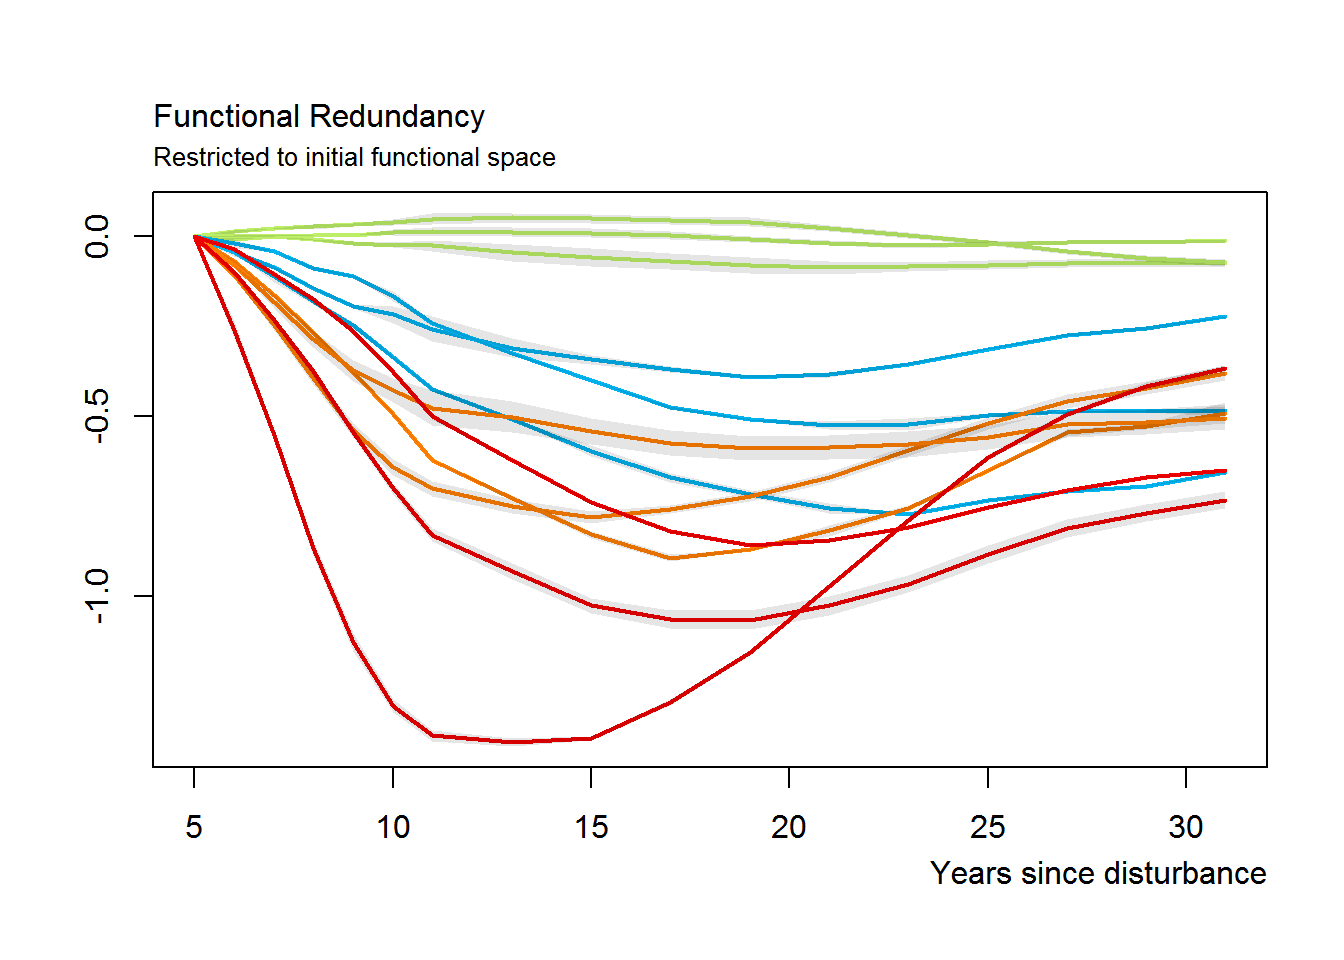
\includegraphics[width=1\linewidth]{WholePlotTrajectories_files/figure-latex/RedFun_rest-1} 

}

\caption{Trajectories of the functional redundancy within the initial cpùùunities functional space over 30 years after disturbance. Trajectories correspond to the median (solid line) and 0.025 and 0.975 percentile (gray envelope) observed after 50 iteration of the taxonomic uncertainty propagation and the missing trait value filling processes. Initial treatments are represented by solid lines colors with green for control, blue for T1,orange for T2 and red for T3.}(\#fig:RedFun_rest)
\end{figure}

\section{Discussion}\label{discussion}

\subsection{Decoupled recovery of communities taxonomic and functional
characteristics}\label{decoupled-recovery-of-communities-taxonomic-and-functional-characteristics}

Both communities taxonomic and functional diversity and composition
proved resilient, following similar humped-back trajectories with a
return towards initial values. The resilience of communities functional
characteristics, the most direct link between biodiversity and ecosystem
functioning \citep{Diaz2005}, meant a consistent recovery of ecosystem
processes in the long term \citep{Guariguata2001}. The resilience of
communities taxonomic characteristics, in turn, meant the maintenance of
their initial differences in composition and structure. It suggested
that communities response to disturbance were somehow constraint to
converge towards determined compositions
\citep{Hubbell1999, Molino2001, Anderson2007, Baraloto2012a}.

Although both communities taxonomic and functional characteristics
proved resilient and followed similar humped-back trajectories, the
taxonomic recovery systematically lagged behind the corresponding
functional dynamics. Such delay between functional and taxonomic
dynamics has already been observed for grasslands
\citep{Tilman1997, Mouillot2011} and more recently for tropical forests
\citep{Lohbeck2015, Guariguata2001}. According to the ``vegetation
quantity effect'' \citep{Grime1998}, functional trajectories rely on the
pool of dominant species which diversity and evenness were enhanced
after disturbance and which rapidly restored the functional diversity
and composition. However, infrequent species that would further lower
the functional diversity and communities evenness still missed to the
recovery of taxonomic characteristics. Taxonomic recovery then
mechanically lagged behind, all the more so that unrecovered species are
functionally redundant and would probably undergo competitive pressures.

\subsection{A validation of the intermediate disturbance
hypothesis}\label{a-validation-of-the-intermediate-disturbance-hypothesis}

The monitoring of disturbed forest communities confirmed a limited or
negative impact of intense disturbance on species richness, as observed
on several post logging surveys \citep{Cannon1998, Baraloto2012a}, while
. Thirty years after disturbance, the genus richness was restored to
initial plot values after high disturbance intensity while it
substantially increased after low disturbance intensity, reaching a gain
of almost 12 genera for some plots.

Both richness and evenness followed asymptotic trajectories after
disturbance, sharply increasing for 15 years before stabilizing at
higher values than those of control plots. An increase of communities
evenness stems from a higher homogeneity of species distribution. After
disturbance, communities are made of the old, pre-disturbance survivors
and the newly recruited trees: changes in composition and abundance
distribution are to be found in the recruitment processes and in the
pre-disturbance survivors mortality. Because the composition of old
survivors proved to mirror the initial community \citep{Herault2018}, a
specific turnover was expected among recruited trees with enhanced
growth and survival of previously infrequent species. Indeed, the
increase in taxonomic diversity was accompanied by an increase of
taxonomic dissimilarity with plots initial state and a functional shift
towards resource-acquisitive strategies (sharp increase in the SLA, leaf
thickness and bark thickness and decrease in wood density, leaf
toughness and maximum height)
\citep{Westoby1998, Wright2004, Reich2014}. Disturbance then causes a
reorganization of the typical high dominance structure of hyperdiverse
mature forests after disturbance, benefiting to pioneers and light
demanding species. Likely, the changes in abiotic environment and
competitive pressure favored pioneers which outcompete others in non
limiting resources but are excluded in mature forests by long-lived,
more resistant and shade tolerant species.

As stated by the IDH, communities dynamics after disturbance relied on
species functional strategy and corresponding ability to fill the
environmental niches made available by disturbance. Recruited species
then mixed with pre-disturbance ones, from which they differed, and
constituted a community all the more diversified that the disturbance
was intense \citep{Molino2001}.

\subsection{Functional redundancy of disturbed
ecosystems}\label{functional-redundancy-of-disturbed-ecosystems}

The functional redundancy, the functional overlap between species that
is typical of the huge biodiversity of tropical forests
\citep{Bellwood2006}, was then not restored 30 years after disturbance
and this is major to consider as it defines forests' resilience
\citep{Trenbath1999, Elmqvist2003, Diaz2005}.

Besides the long-term alteration of functional redundancy, there was
probably persistent compositional changes favoring disturbance resistant
species \citep{Haddad2008}, lianas or epiphytes \citep{Martin2013} and
environmental changes, like in the soils nutrient cycling and compaction
\citep{Olander2005}. These persistent changes highly question forest's
resilience \citep{Chazdon2003a}. New conditions would not only be longer
lasting but self-maintained as tied to disturbance regime
\citep{Burslem2000}. Specificaly, this would impair species contingent
to undisturbed forests, threatening their maintenance, and run the risk
to loose cornerstone species and trigger unexpected ecological
consequences \citep{Jones1994, Diaz2005, Gardner2007}.

\section{Conclusions}\label{conclusions}

Our study showed the significant impact of disturbance on tropical
forests communities and validated the consistency of the IDH in the long
term. It revealed the contrasting response of communities taxonomic and
functional characteristics, with persisting impacts on the species
abundance distibution while the functional diversity and dominant
functional strategies were restored. Communities recovery therefore
remained unachieved but consistent for the range of disturbance studied
here. The length of the recovery, however, severly questioned the
sustainability of intense selective logging and advocated felling cycle
much longer than 30 years \citep{Gourlet-Fleury2005}.

%----------------------------------------------------------------------------------------
%	REFERENCE LIST
%----------------------------------------------------------------------------------------

\bibliographystyle{mee}
\makeatletter
% The filename has .bib extension the must be eliminated
\filename@parse{references.bib}
% parse stores the file name in base. Extension starts at the first dot, so don't use dots in file names.
\bibliography{\filename@base}
\makeatother


%----------------------------------------------------------------------------------------

\end{document}
